\section{Auswertung}
Zu Anfang wird die Leerlaufsannung einer Monozelle bestimmt
und der Innenwiderstand vom Amperemeter abgelesen.
\begin{align*}
  U &= 1,47\, \mathrm{V} & R_I &= 10\, \mathrm{M\Omega}
\end{align*}
Im folgenden werden für die drei Spannungsquellen die Spannung $U_0$ und
der Widerstand $R_i$ bestimmt.
Dafür werden die gemessenen Werte für die Klemmspannung $U_k$
gegen die Werte für den Strom $I$ aufgetragen.
Diese Werte sind in den Tabellen (\ref{tab:1}), (\ref{tab:2}), (\ref{tab:3})
und (\ref{tab:4}) zu finden.
Der Wert für die Steigung der folgenden linearen Ausgleichsgraden,
beschreibt den Wert des Innenwiderstandes. Die Verschiebung auf der y-Achse
beschreibt den Wert für $U_0$
\subsection{Monozelle ohne Gegenspannung}
Die Werte für $R_i$ und $U_0$ für eine Monozelle ohne Gegenspannung,
werden wie oben beschrieben ermittelt und lauten:
\begin{align}
  R_i &= (15,60 \pm 0,16)\, \mathrm{\Omega}\\
  \label{eqn:ri}
  U_0 &= (1,519 \pm 0,008)\, \mathrm{V}
\end{align}
Die Regression ist in Abbidung (\ref{fig:Messunga}) zu sehen.
\begin{table}
  \centering
  \caption{Messwerte für eine Monozelle ohne Gegenspannung}
  \label{tab:1}
  \begin{tabular}{c c }
    \toprule $I/A$ & $U/V$ \\
    \midrule
    0,092 & 0,09\\
    0,070 & 0,42\\
    0,059 & 0,60\\
    0,0495 & 0,75\\
    0,043 & 0,84\\
    0,037 & 0,93\\
    0,033 & 1,02\\
    0,029 & 1,05\\
    0,027 & 1,11\\
    0,024 & 1,14\\
    0,023 & 1,17\\
    \bottomrule
  \end{tabular}
\end{table}

\begin{figure}[H]
  \centering
  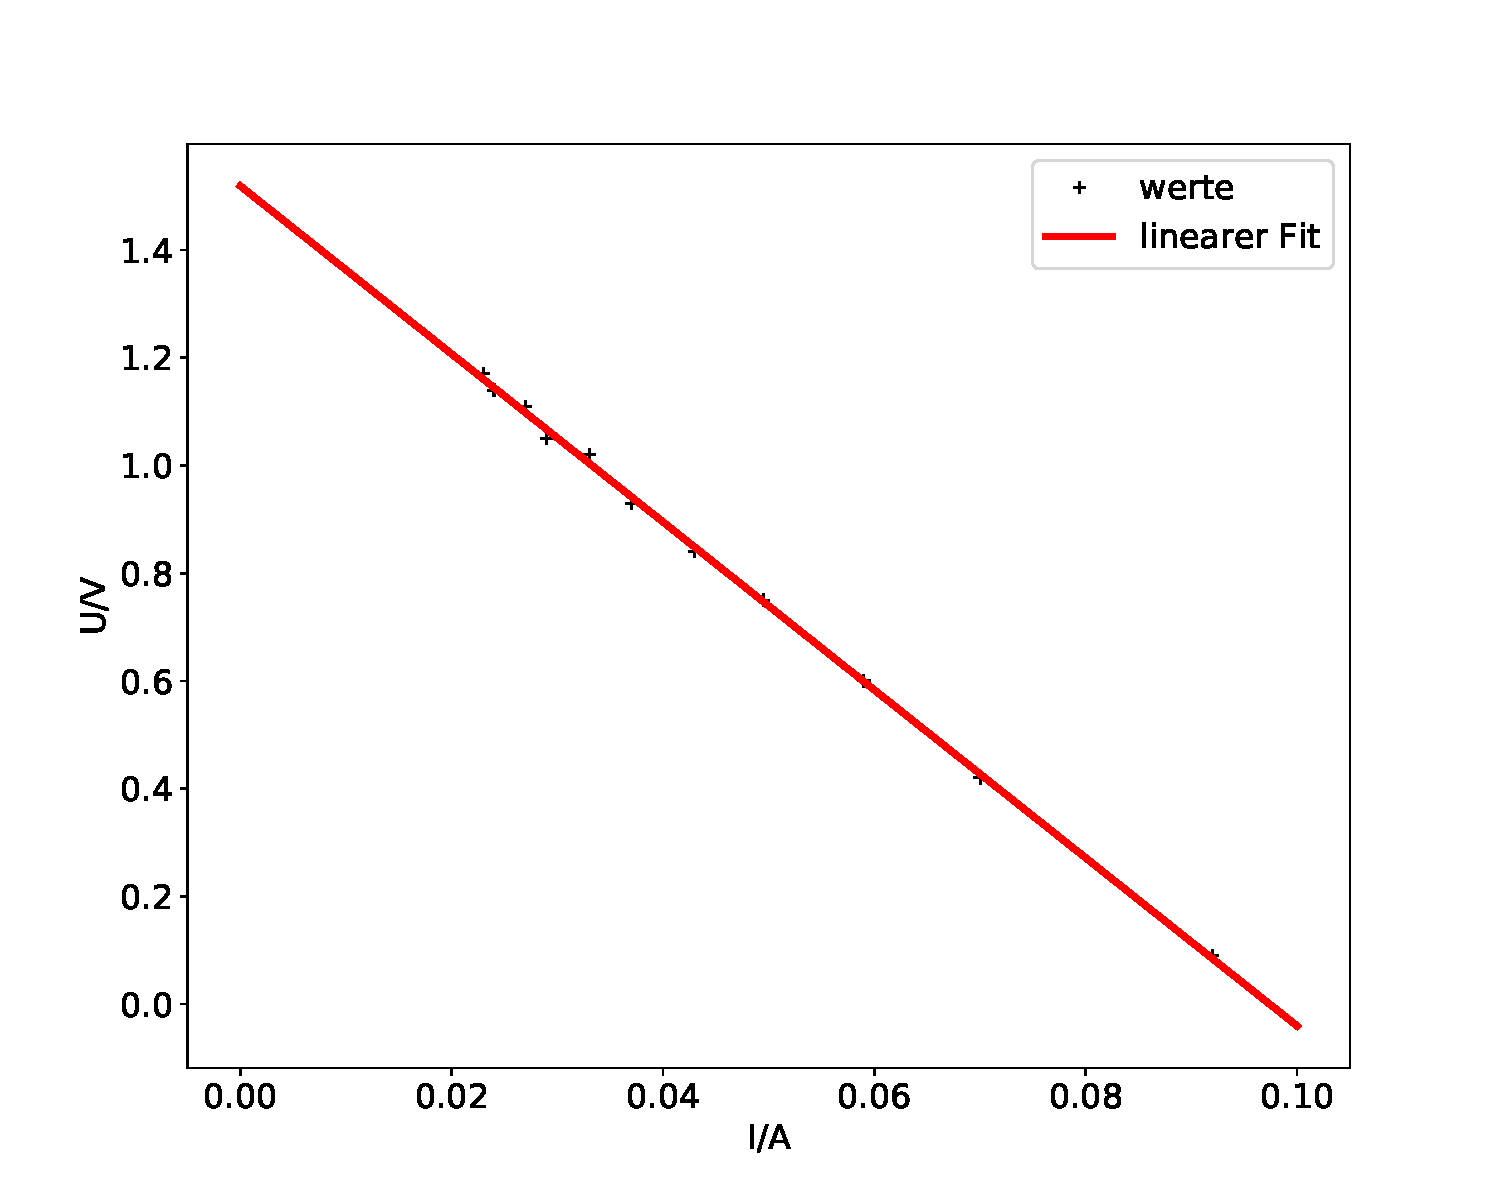
\includegraphics[width=\textwidth]{plota.pdf}
  \caption{Monozelle ohne Gegenspannung}
  \label{fig:Messunga}
\end{figure}
\subsection{Monozelle mit Gegenspannung}
Ist an der Monozelle eine Gegenspannung angelegt,
ergeben sich folgende Werte für $R_i$ und $U_0$:
\begin{align*}
  R_i &= (4,80 \pm 0,22)\, \mathrm{\Omega}\\
  U_0 &= (0,467 \pm 0,013)\, \mathrm{V}
\end{align*}
Die lineare Regression ist in Abbildung (\ref{fig:Messungb}) gezeigt.
\begin{table}
  \centering
  \caption{Messwerte für eine Monozelle mit Gegenspannung}
  \label{tab:2}
  \begin{tabular}{c c}
    \toprule $I/mA$ & $U/V$ \\
    \midrule
    99 & 0,96\\
    91 & 0,87\\
    68 & 0,81\\
    58 & 0,75\\
    51 & 0,72\\
    46 & 0,69\\
    41 & 0,66\\
    37 & 0,64\\
    34 & 0,63\\
    33 & 0,62\\
    \bottomrule
  \end{tabular}
\end{table}

\begin{figure}[H]
  \centering
  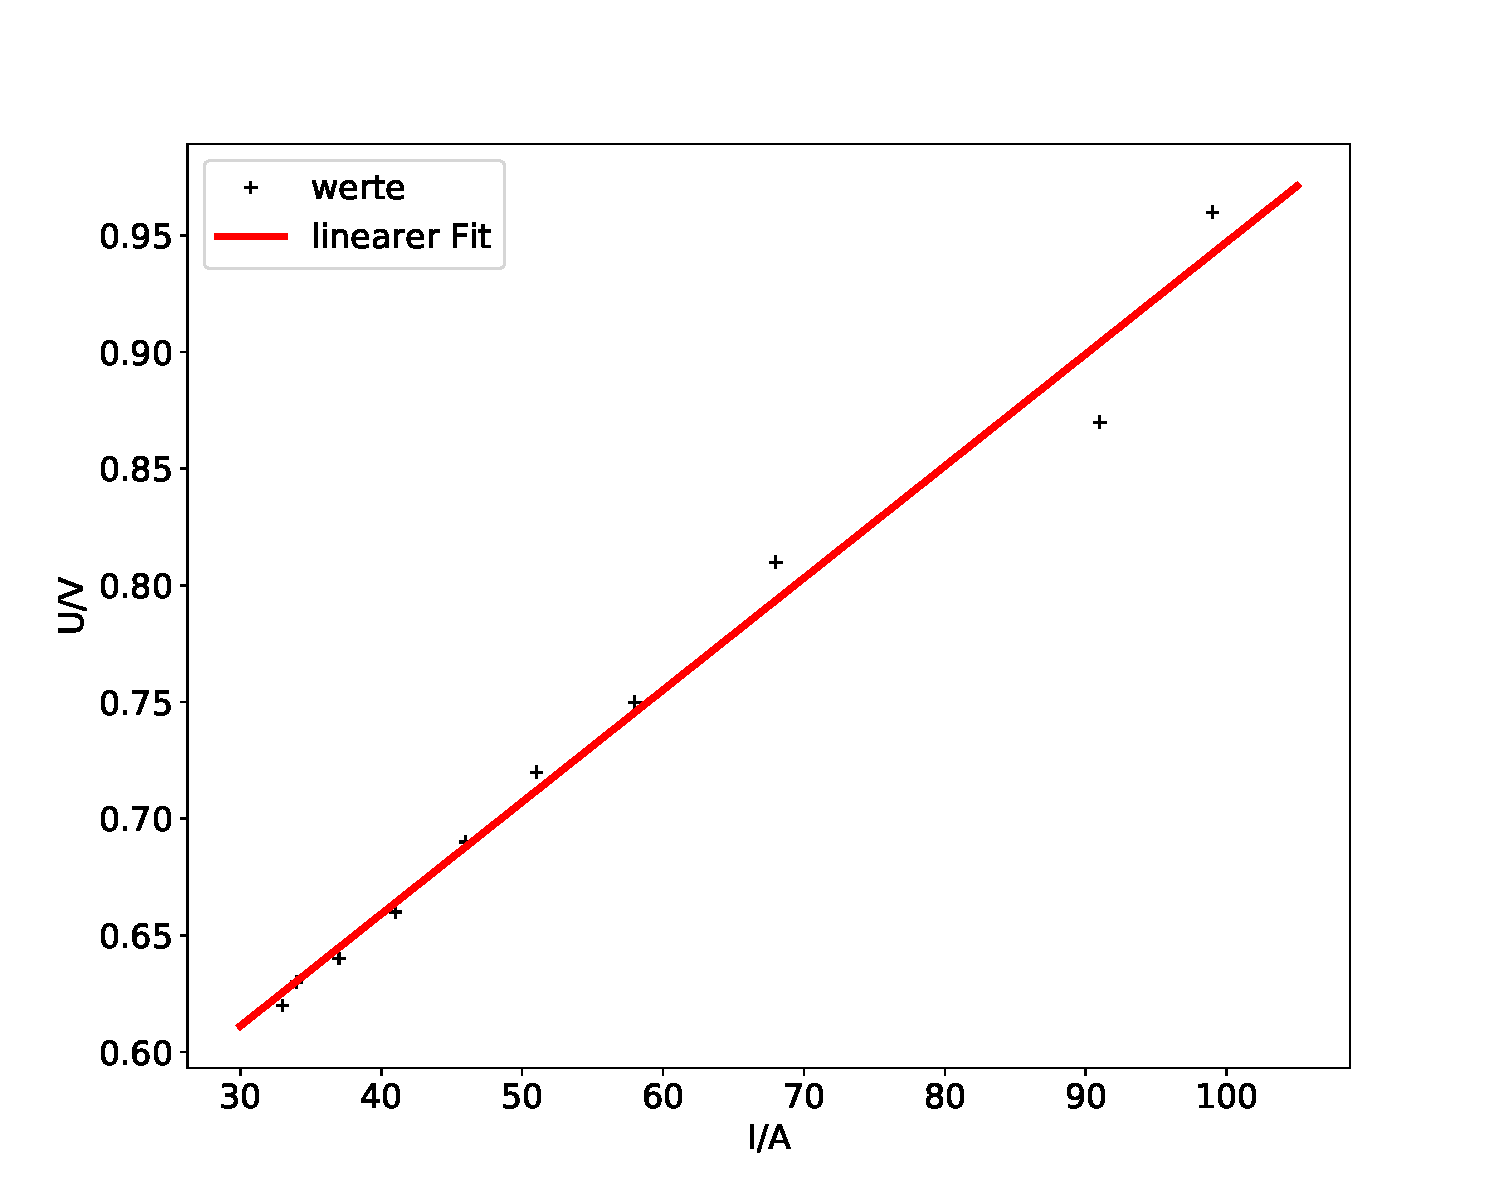
\includegraphics[width=\textwidth]{plotb.pdf}
  \caption{Monozelle mit Gegenspannung}
  \label{fig:Messungb}
\end{figure}

\subsection{Rechteck- und Sinusspannung}
Für die Rechteck- und Sinusspannung wird die Regression
und die Bestimmung von $U_0$ und $R_i$ ebenfalls wie oben bestimmt.
\begin{table}
  \centering
  \caption{gemessene Werte zur Rechteckspannung}
  \label{tab:3}
  \begin{tabular}{c c}
    \toprule $I/mA$ & $U/V$  \\
    \midrule
    8,0 & 0,19\\
    7,1 & 0,23\\
    5,7 & 0,32\\
    4,4 & 0,38\\
    3,6 & 0,42\\
    3,2 & 0,45\\
    2,8 & 0,47\\
    2,5 & 0,49\\
    2,2 & 0,50\\
    2,0 & 0,52\\
    1,8 & 0,53\\
    \bottomrule
  \end{tabular}
\end{table}
Für die Rechteckspannung lauten die Werte:
\begin{align*}
  R_i &= (54,8 \pm 0,8)\, \mathrm{\Omega}\\
  U_0 &= (0,6249 \pm 0,0034)\, \mathrm{V}
\end{align*}
Die Regression ist in Abbildung (\ref{fig:c}) zu sehen.

\begin{figure}[H]
  \centering
  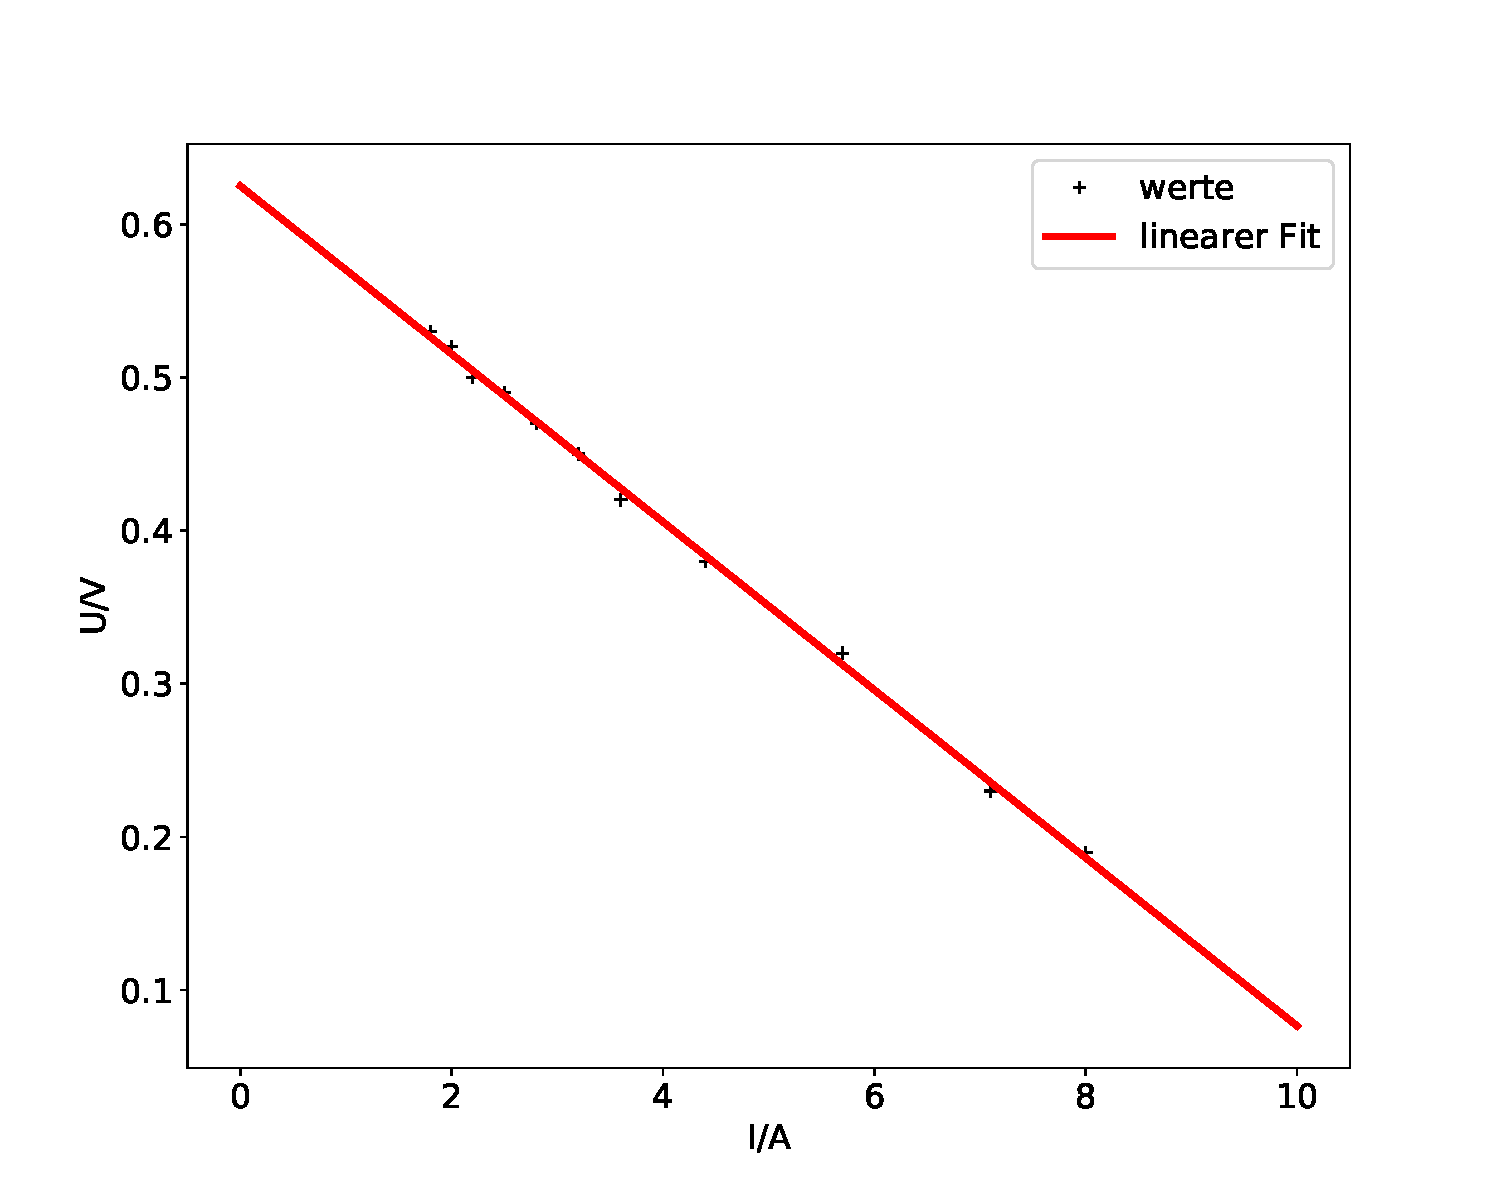
\includegraphics[width=\textwidth]{plotreck.pdf}
  \caption{Monozelle ohne Gegenspannung}
  \label{fig:c}
\end{figure}

\begin{table}
  \centering
  \caption{gemessene Werte zur Sinusspannung}
  \label{tab:4}
  \begin{tabular}{c c}
    \toprule $I/mA$ & $U/V$  \\
    \midrule
    0,97 & 0,41\\
    0,66 & 0,62\\
    0,50 & 0,73\\
    0,39 & 0,81\\
    0,34 & 0,85\\
    0,28 & 0,88\\
    0,24 & 0,91\\
    0,20 & 0,94\\
    0,18 & 0,96\\
    0,16 & 0,97\\
    \bottomrule
  \end{tabular}
\end{table}
Die Werte für die Sinusspannung lauten:
\begin{align*}
  R_i &= (693 \pm 5)\, \mathrm{\Omega}\\
  U_0 &= (1,0795 \pm 0,0024)\, \mathrm{V}
\end{align*}
die lineare Regression ist in Abbildung (\ref{fig:d}) gezeigt.
  \begin{figure}[H]
    \centering
    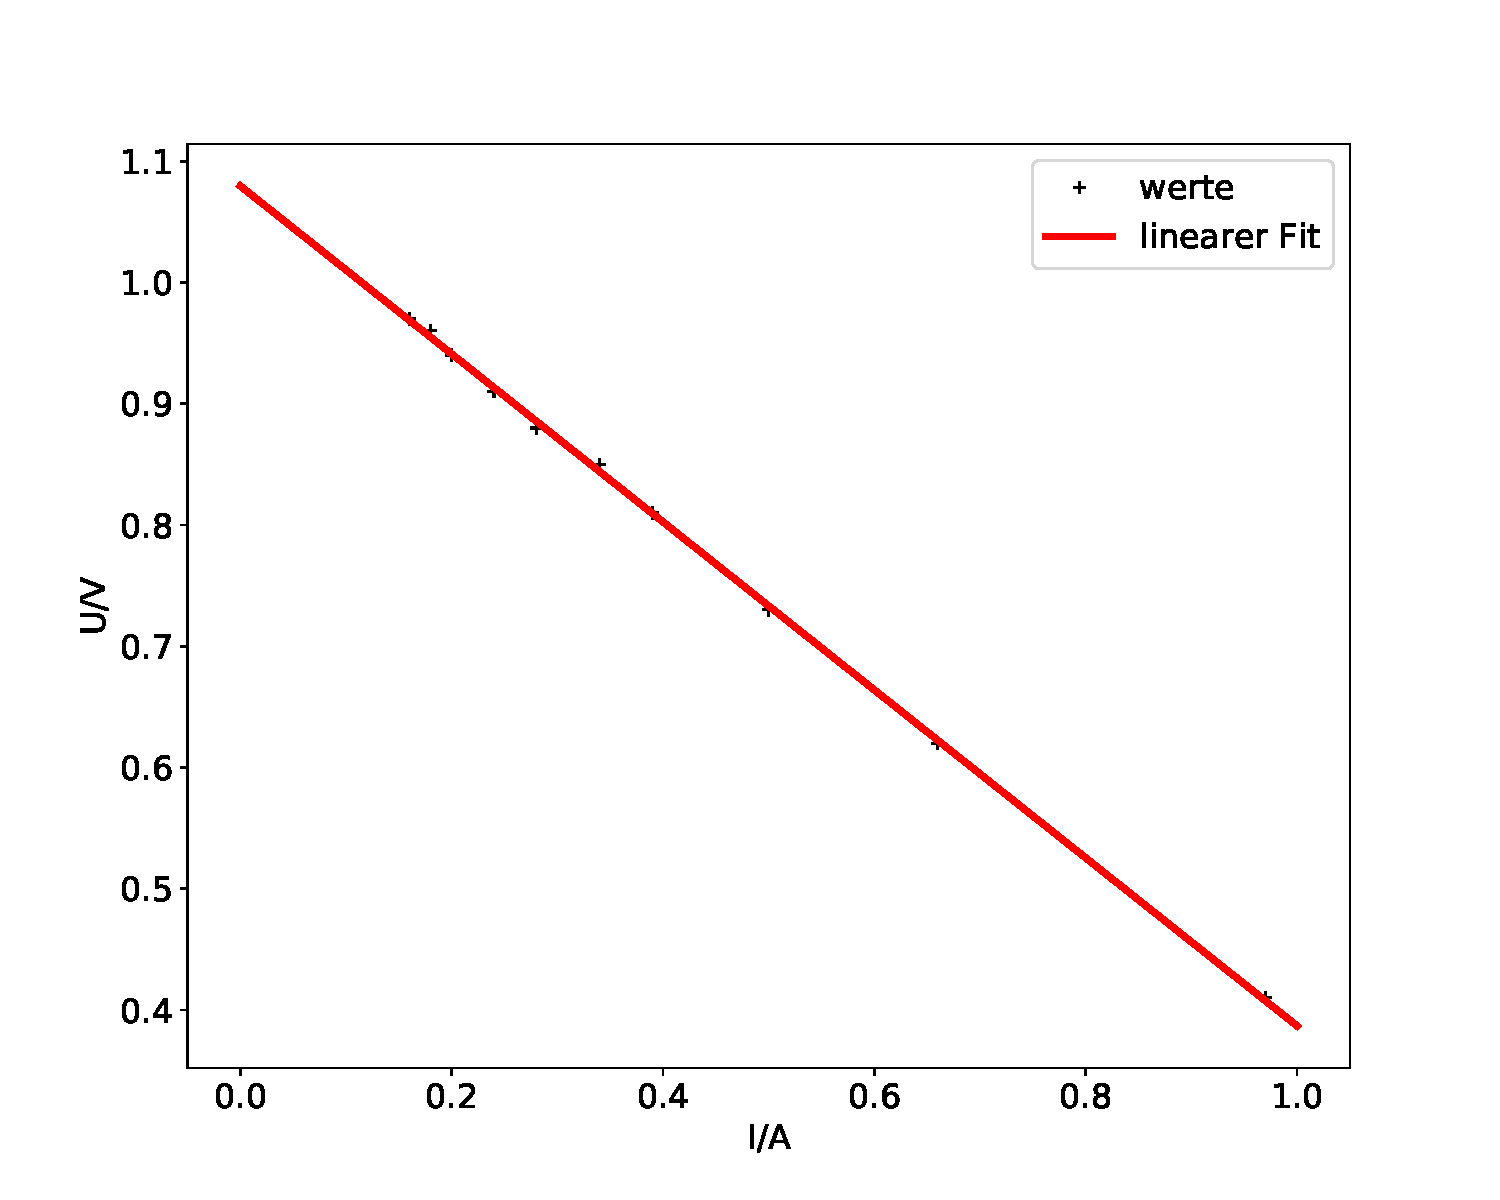
\includegraphics[width=\textwidth]{plotsin.pdf}
    \caption{Monozelle ohne Gegenspannung}
    \label{fig:d}
  \end{figure}
Die verwendeten Messwerte sind in den Tabellen (\ref{tab:3}) und (\ref{tab:4}) zu finden.

  \subsection{Systematischer Fehler der $U_0$ Messung}

Der systematische Fehler der $U_0$-Messung entsteht aufgrund des Eigenwiderstandes
des verwendeten Voltmeters.
Dieser wird vom Gerät abgelesen und liegt bei $10\, M\Omega$
Der Fehler wird mit der Formel
\begin{equation}
  \Delta U = U_K \cdot \frac{R_i}{R_v}\,\, := f
\end{equation}
berechnet. $U_K$ ist die Klemmspannung und wurde zu Anfang abgelesen.
Sie liegt bei $1,47 \, V$. \\
$R_i$ entspricht den in \ref{eqn:ri} berechneten Innenwiderstand.
\\
Der fehler ergibt sich durch Formel:
\begin{equation*}
  \Delta f = \frac{U_K}{R_v}\cdot\Delta R_i
\end{equation*}
Somit berechnet sich der Fehler zu
\begin{equation*}
  \Delta U = (2,2932 \pm 0,0235) \cdot 10^{-6} \mathrm{V}\, .
\end{equation*}

\subsection{Im Belastungswiderstand umgesetzte Leistung der Monozelle}
Die im Belastungswiderstand umgesetzte Leistung wird ermittelt,
indem $U \cdot I$ gegen $U/I$ aufgetragen wird.
Die Werte sind in Tabelle (\ref{tab:lei}) zu finden.
\begin{table}
  \centering
  \caption{n}
  \label{tab:lei}
  \begin{tabular}{c c c c}
    \toprule $I/A$ & $U/V$ & $(U\cdot I)/W$ & $(U/I)/\Omega$\\
    \midrule
    0,092 & 0,09 & 0,0083 & 0,978\\
    0,070 & 0,42 & 0,0294 & 6,00\\
    0,059 & 0,60 & 0,0354 & 10,17\\
    0,0495 & 0,75 & 0,0371 & 15,15\\
    0,043 & 0,84 & 0,0361 & 19,53\\
    0,037 & 0,93 & 0,0344 & 25,14\\
    0,033 & 1,02 & 0,0337 & 30,90\\
    0,029 & 1,05 & 0,0305 & 36,21\\
    0,027 & 1,11 & 0,0299 & 41,11\\
    0,024 & 1,14 & 0,0274 & 47,50\\
    0,023 & 1,17 & 0,0269 & 50,87\\
    \bottomrule
  \end{tabular}
\end{table}
In Abbildung (\ref{fig:fite}) sind die Werte aufgetragen.
Außerdem wurde eine Theoriekurve mit der Formel
\begin{equation*}
  N(R_a)= \frac{ U_0^2 \cdot R_a}{(R_i + R_a)^2}
\end{equation*}
eingefügt, um systematische Fehler zu ermitteln.
\begin{figure}[H]
  \centering
  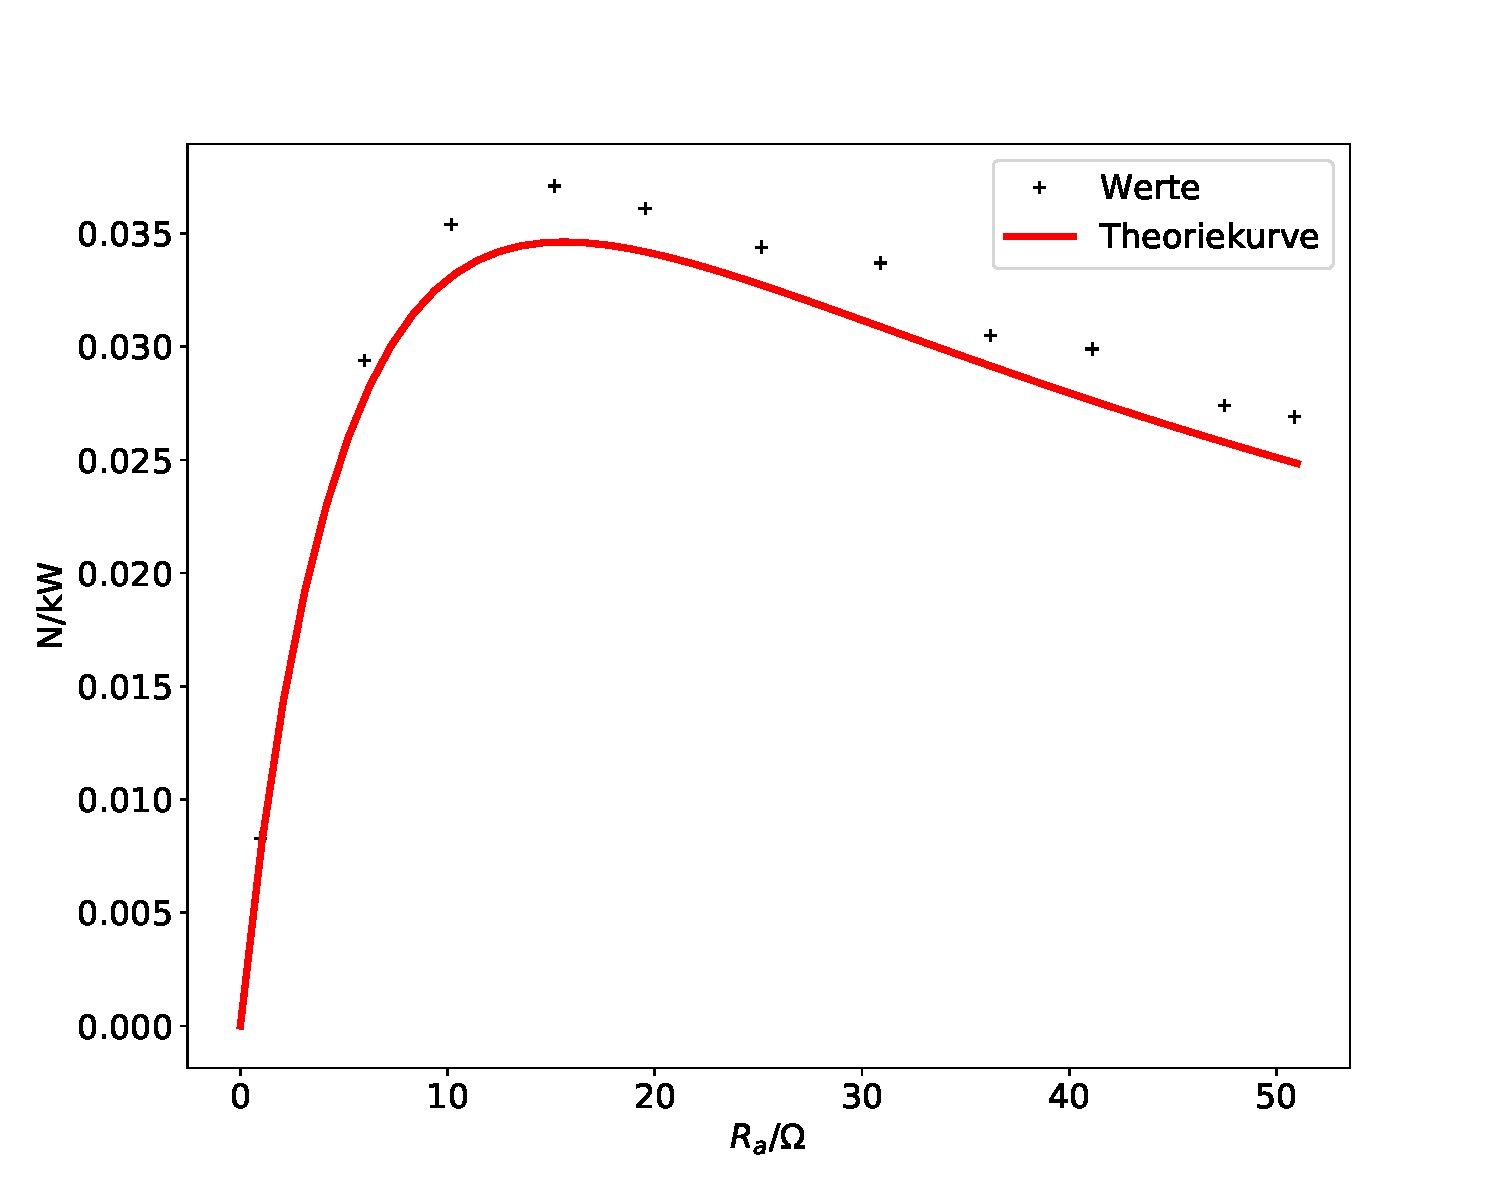
\includegraphics[width=\textwidth]{plote.pdf}
  \caption{Leistungsabfall am Belastungswiderstand}
  \label{fig:fite}
\end{figure}
Die meisten Messwerte liegen über der Kurve.
Allerdings liegt die abweichung bei ca. $0,002\, V$, sodass nicht davon auszugehen ist,
dass  ein systematischer Fehler gemacht wurde.
Das Maximum der Kurve liegt vor, wenn $R_a = R_i$
und stimmt sehr gut mit den gemessenen Werten überein.

\section{Diskussion}

In den Abbildungen der linearen Regressionen ist gut zu erkennen,
dass die Messwerte gegenüber der Ausgleichsgrade nur leicht Abweichen
und im Bereich der Messungenauigkeiten liegen.
somit ist davon auszugehen, dass keine größeren Systematischen Fehler begangen wurden.
Es fällt allerdings auf, dass die gemessene Spannung $U_0$ und der Widerstand $R_i$ einer Monozelle
 mit Gegenspannung sehr klein sind.
 Dieses Ergebnis wurde nicht erwartet und könnte an einem Fehler im Aufbau der Schaltung liegen.
 Das Amperemeter sollte hinter das Voltmeter geschaltet werden.
 Wird dieses andersherum aufgebaut, wirkt der Eigenwiderstand des Amperemeter
 und verringert den Wert der Messung sehr stark.
